\begin{frame}{Rise of Diffusion Models}
\begin{figure}
\includegraphics[width=.8\linewidth]{images/stablediffusion.jpg}
\caption{Samples from stable diffusion}
\end{figure}
\end{frame}

\begin{frame}{Goal}
{Build probabilistic model over feature fields $f: \mathcal{X} \rightarrow \mathcal{Y}$.}
\begin{figure}
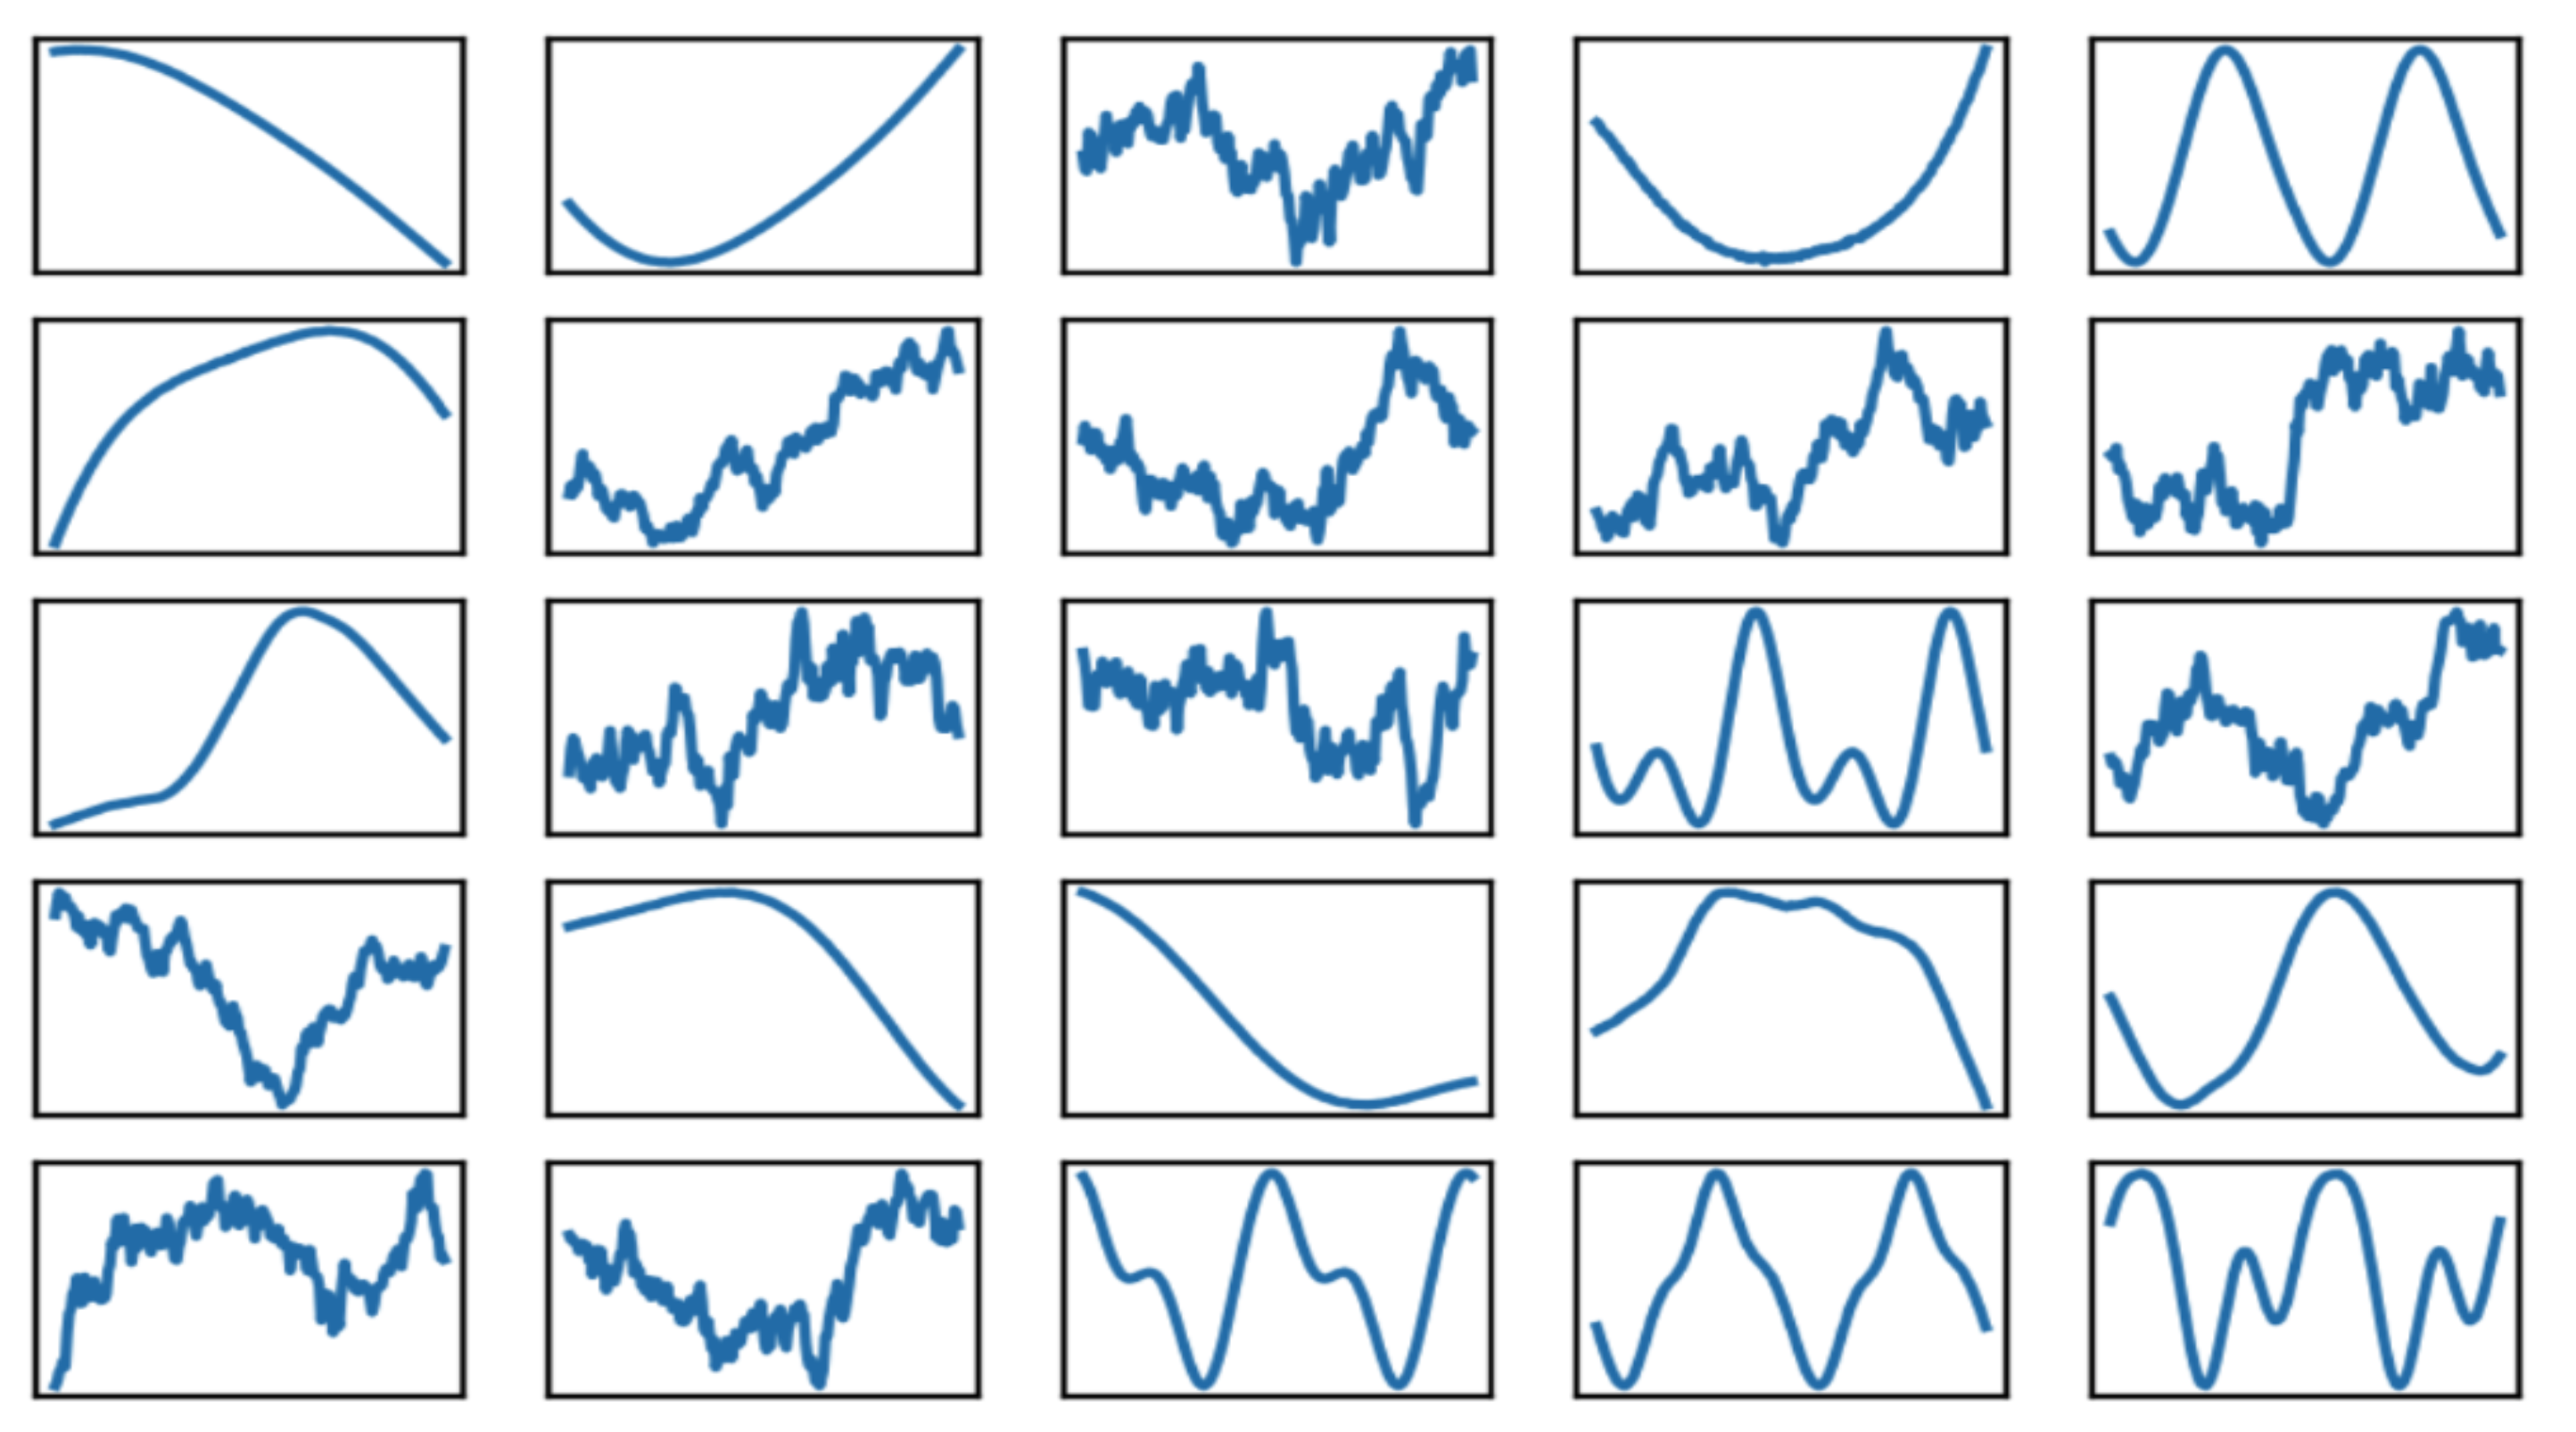
\includegraphics[width=.7\linewidth]{images/functions}
\end{figure}
\pause
\vspace{-5mm}
\textbf{Why}
\begin{itemize}
    \item Many physical and natural phenomena are better characterised as functions.
    \item Meta-learn and treat limited data as originating from a function.
\end{itemize}
\end{frame}

\begin{frame}{Feature Fields: $f: \mathcal{X} \rightarrow \mathbb{R}^d$}

\begin{itemize}
    \item Mathematical framework for modelling natural phenomena.
    \item Examples: Temperature $f:\mathcal{X}\rightarrow\mathbb{R}$,
    and wind direction on globe $f:\mathcal{S}^2\rightarrow T\mathcal{S}^2$.
\end{itemize}

    % \begin{itemize} 
    %     \item Build a probabilistic model over feature fields $f: \mathcal{X} \rightarrow \mathcal{Y}$
    %     \item Encode invariances w.r.t. group transformations $p(f) = p(g\cdot f),\ \forall g \in G$.
    % \end{itemize}
    % \textbf{Examples:}
    \begin{figure}
        \centering
        \begin{subfigure}{0.45\textwidth}
            \centering
            \includegraphics[width=0.95\textwidth]{images/geomndp/tensors/salinity_and_current}
            \caption{Temperature map and wind vector fields.}
        \end{subfigure}
        \hfill
        \begin{subfigure}{0.45\textwidth}
            \centering
            \includegraphics[width=0.95\textwidth]{images/geomndp/tensors/stress_wiki.png}
            \caption{3D stress tensor (type-2) diagram.}
        \end{subfigure}
    \end{figure}
\end{frame}

\begin{frame}{Prior invariances}
Encode invariances w.r.t. group transformations. For a group $G$, we want $\forall g \in G$
\begin{equation*}
p(f) = p(g\cdot f) \quad\text{with}\quad g \cdot f = \rho(g) f (g^{-1} x).
\end{equation*}
\pause
\textbf{Examples} translation invariance (stationarity) and rotational invariance.
\begin{figure}[t]
\centering
\begin{subfigure}[b]{0.45\textwidth}
\centering
\includegraphics[width=1.\linewidth,trim={0 0 0 0},clip]{images/geomndp/1d/prior_ndp_shift.pdf}
% \caption{$G=T(1)$}
\end{subfigure}%
\hspace{0.3cm}
\begin{subfigure}[b]{0.45\textwidth}
\centering
\includegraphics[width=1.\linewidth,trim={0 0 0 0},clip]{images/geomndp/2d/prior_ndp_rot.pdf}
% \caption{$G=O(2)$}
\vspace{-.75em}
\end{subfigure}
\label{fig:prior_model}
\end{figure}
% \item We get these properties for free in most GP kernels.
% \item How can we encode them in our diffusion models on funcions?
\end{frame}

\begin{frame}{Conditional process}
\begin{itemize}
    \item Interested in the conditional process given a
    set of observations $\mathcal{C} = \{(x_n, y_n)\}_{n=1}$.
\item If the prior is $G$-invariant, then the conditional is $G$-equivariant:
    $$
    p(f \mid \mathcal{C}) = p(g\cdot f| g \cdot \mathcal{C})
    \quad\text{where}\quad g \cdot \mathcal{C} = \{(g \cdot x_n, \rho(g) y_n) \}.
    $$
\end{itemize}
\begin{figure}[t]
% \begin{wrapfigure}[20]{r}{.5\linewidth}
    % \vspace{-1em}
    \centering
        \begin{subfigure}[b]{0.49\textwidth}
        \centering
        \vspace{0.em}
        \includegraphics[width=1.\linewidth,trim={0 0 0 0},clip]{images/geomndp/1d/conditional_ndp_shift.pdf}
    % \includegraphics[width=.48\linewidth,trim={0 0 0 0},clip]{../figs/1d_conditional.png}
    % \includegraphics[width=.48\linewidth,trim={0 0 0 0},clip]{../figs/1d_conditional_shift.png}
        \end{subfigure}
        \begin{subfigure}[b]{0.49\textwidth}
        \centering
        \vspace{0.em}
    \includegraphics[width=1.\linewidth,trim={0 0 0 0},clip]{images/geomndp/2d/conditional_ndp_rot.pdf}
    % \includegraphics[width=.48\linewidth,trim={40em 0 0 0},clip]{../figs/conditional_ndp_rot.png}
    %  \includegraphics[width=.48\linewidth,trim={4em 0 36em 0},clip]{../figs/conditional_ndp_rot.png}
    \vspace{-.75em}
    % \vfill
    \end{subfigure}
    \vspace{-0.5em}
    % \caption{
    % Samples from equivariant neural diffusion processes conditioned on context set $\mathcal{C}$ (\textcolor{C3}{in red}) for scalar (\emph{Left}) and 2D vector (\emph{Right}) fields.
    % Same model is then conditioned on transformed context $g \cdot \mathcal{C}$. %, with group element $g$ being a translation of length $2$ (\emph{Left}) or a $90^{\circ}$ rotation (\emph{Right}).
    % }
    \label{fig:posterior_model}
\end{figure}
\end{frame}